\documentclass[a4paper, 12pt]{article}%тип документа

%отступы
\usepackage[left=1.5cm,right=1cm,top=2cm,bottom=3cm,bindingoffset=0cm]{geometry}
\setlength{\parindent}{5ex}

%Русский язык
\usepackage[T2A]{fontenc} %кодировка
\usepackage[utf8]{inputenc} %кодировка исходного кода
\usepackage[english,russian]{babel} %локализация и переносы

%Вставка картинок
\usepackage{graphicx}
\graphicspath{{pictures/}}
\DeclareGraphicsExtensions{.pdf,.png,.jpg,}
\usepackage{wrapfig}

%Графики
\usepackage{pgfplots}
\pgfplotsset{compat=1.9}

%Математика
\usepackage{amsmath, amsfonts, amssymb, amsthm, mathtools}

%Таблицы
\usepackage{longtable} 
\usepackage{float}

%Римские цифры
\newcommand{\RomanNumeralCaps}[1]{\uppercase\expandafter{\romannumeral#1}}

\usepackage{multirow}


\begin{document}
	\begin{titlepage}
		\begin{center}
			\textsc{Федеральное государственное автономное образовательное учреждение высшего образования«Московский физико-технический институт (национальный исследовательский университет)»\\[5mm]
			}
			
			\vfill
			
			\textbf{Вопрос по выбору: \\[3mm]
				Закон Мозли.
				\\[50mm]
			}
			
		\end{center}
		
		\hfill
		\begin{minipage}{.5\textwidth}
			Выполнили студенты:\\[2mm]
			Сериков Василий Романович\\[2mm]
			Группа: Б03-102\\[5mm]
			Сериков Алексей Романович\\[2mm]
			Группа: Б03-102\\[5mm]
			
		\end{minipage}
		\vfill
		\begin{center}
			Москва, 2023 г.
		\end{center}
		
	\end{titlepage}
	
	\newpage
	\textbf{Аннотация}\\
	
	В работе измеряются спектры характеристического излучения
	атомов некоторых химических элементов. Определяются рентгеновские
	термы измеренных спектральных пиков излучения. Проверяется закон Мозли.\\
	
	\textbf{Теоретические сведения: }\\
	
	Энергетический спектр состояний электрона в
	атоме водорода имеет вид (СГС):
	
	\begin{equation}
		E_n=-\frac{m e^4}{2 \hbar^2} \frac{1}{n^2}=-R \frac{1}{n^2}
	\end{equation}
	
	где R – постоянная Ридберга, выраженная в энергетических единицах, m – масса электрона, e – элементарный заряд, $\hbar$ – постоянная
	Планка, n – положительное целое число, означающее номер стационарного уровня энергии
	
	
	Заданное состояние, относящееся к одному энергетическому уровню, помимо номера n определяется значениями момента импульса (орбитальный момент) и его проекции на выбранное направление.
	
	
	Номер уровня
	n называют главным квантовым числом, а целые числа, определяющие
	в единицах $\hbar$ величину орбитального момента и его проекцию на выделенное направление, обозначают l и m соответственно. Полный
	набор из 4 квантовых чисел: n, l, $m_l$
	, $m_s$, где $m_l$ – определяет проекцию
	орбитального момента на некоторое выделенное направление (ось z), а
	$m_s$ – проекцию спинового момента на ту же ось z.
	
	
	Такое описание сложно обобщить на случай многоэлектронных атомов, поэтому применяется другой, более подходящий, набор квантовых чисел. Вместо отдельного рассмотрения орбитального и спинового моментов вводится полный момент импульса j, а также проекция
	полного момента $m_j$ на выделенную ось. Полный момент импульса –
	это векторная сумма орбитального и спинового моментов, поэтому его
	величина может принимать значения в диапазоне от |l - s| до l + s.
	
	
	Строгий учёт спина у электрона возможен при решении задачи об
	атоме водорода с помощью релятивистского уравнения Дирака. Наличие спина у электрона приводит к возникновению спин-орбитального
	взаимодействия, которое, тем не менее, можно учитывать, оставаясь в рамках нерелятивистской теории. Важным результатом такого взаимодействия является то, что электрон в состоянии, соответствующем заданному уровню энергии, также обладает
	определённым полным моментом импульса j. То есть энергия состояния
	оказывается зависящей не только от главного квантового числа n, но
	и от величины полного момента j, что приводит к тонкому расщеплению уровней энергии, определяемых формулой (1). 
	
	
	Атомы химических элементов, отличных от водорода, включают в
	себя более чем один электрон, и их описание возможно только приближёнными методами, поскольку электроны взаимодействуют не только
	с ядром атома, но и друг с другом. При этом, помимо электрического взаимодействия как такового, следует учитывать важнейший фактор квантовой статистики электронов – запрет Паули, который тесно
	связан с требованием антисимметричности волновой функции системы
	фермионов (частиц с полуцелым спином) по отношению к парным перестановкам этих частиц.
	Так, если описывать некоторый многоэлектронный
	атом, пренебрегая взаимодействием между электронами и не учитывая
	спин электронов, то для каждого электрона в отдельности получится система энергетических уровней, описываемых формулой, аналогичной
	формуле (1), но с учётом заряда ядра Z:
	
	\begin{equation}
		E_n=-\frac{m Z^2 e^4}{2 \hbar^2} \frac{1}{n^2}=-R \frac{Z^2}{n^2}
	\end{equation}
	
	Такой спектр энергетических уровней называют водородоподобным. Полученный таким
	способом результат для многоэлектронного атома не даст количественного согласия с экспериментальными данными, поскольку межэлектронное
	взаимодействие вносит существенный вклад.
	
	Для уточнения этой модели необходимо учесть межэлектронное, спин-орбитальное. Межэлектронное электростатическое взаимодействие оказывает наиболее существенное влияние
	на величину энергетических уровней.
	Приближённо учёт электростатического межэлектронного взаимодействия можно провести следующим образом. Для заданного электрона,
	находящегося в некотором состоянии (n, l, m), суммарное действие всех
	других электронов, в основном сводится к частичному экранированию
	заряда ядра. Величина этого экранирования зависит от количества электронов, средние радиусы оболочек которых меньше либо равны радиусу оболочки (nl). Можно ввести константу экранирования $\sigma_{n, l}$, так что
	формула (2) примет вид:
	
	\begin{equation}
		E_n=-\frac{m (Z - \sigma_{n, l})^2 e^4}{2 \hbar^2 n^2}=-R \frac{(Z - \sigma_{n, l})^2}{n^2}
	\end{equation}

	\addvspace{20pt}

	\textit{Излучательные переходы и рентгеновские термы}\\
	
	Нас будут интересовать переходы между возбуждёнными состояниями атома, обусловленные переходами электронов между различными состояниями с малыми значениями главного квантового
	числа n. Для возможности таких переходов необходимо наличие свободного электронного состояния на глубоком уровне, то есть необходимо
	предварительно освободить это состояние. Это
	можно сделать за счёт поглощения фотона с достаточно большой энергией. Образовавшееся свободное электронное состояние приводит к тому,
	что соответствующая электронная оболочка (nl) становится частично заполнена, и она приобретает момент импульса j = l $\pm 1/2$
	освободившегося
	электронного состояния. При этом энергия атома повышается на величину, равную энергии связи удалённого электрона, которая может быть
	приблизительно расчитана по формуле (3). Уровни энергии атома, у
	которого удалён один из электронов с глубокого уровня, называют рентгеновскими термами
	
	
	При переходе электрона с оболочки одного слоя на другой слой атом
	излучает рентгеновский квант, такое излучение называют характеристическим излучением. Энергия кванта такого излучения приближённо
	может быть записана в виде:
	
	\begin{equation}
		\hbar \omega_{12}=E_{n_2}-E_{n_1}=-R y\left(\frac{\left(Z-\sigma_{n_2, l_2}\right)^2}{n_2^2}-\frac{\left(Z-\sigma_{n_1, l_1}\right)^2}{n_1^2}\right),
	\end{equation}

	формула (4), является приближённой,
	но она отражает основное свойство спектральных линий характеристического излучения: квадратичную зависимость частоты излучения от заряда ядра Z – аналогично тому как это имеет место в водородоподобном спектре. Основным подтверждением формулы (5) является
	хорошее совпадение с экспериментом. Именно такая зависимость
	была впервые экспериментально обнаружена Мозли в 1913 году.\\
	
	
	\textbf{Экспериментальная установка: }\\
	
	Для регистрации рентгеновских спектров характеристического излучения в работе используется серийно выпускаемый рентгенофлуоресцентный спектрометр «Спектроскан Макс-G». В состав прибора входят следующие основные элементы: рентгеновская трубка, держатель образцов,
	вогнутая пластина кристалла LiF (Фторид лития), гониометр, а также пропорциональный детектор. Схема прибора показана на рис. 1.
	
	\begin{figure}[H]
		\center{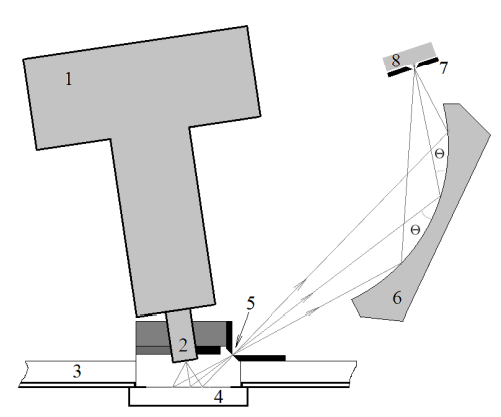
\includegraphics[scale=1.1]{ust.png}}
		\caption{Схема рентгеновского спектрометра}
	\end{figure}
	
	Рентгеновская трубка 1
	установлена так, что её носик 2 с выходным окном располагается непосредственно над поверхностью анализируемого образца 4. Образец подаётся ниже основного днища прибора 3 с помощью специального механизма. Рентгеновское излучение образуется за счёт торможения разогнанных электронов в тонком слое меди, которая нанесена на бериллиевую пластинку, прозрачную для рентгеновских лучей. Непрерывное
	тормозное излучение трубки «освещает» на поверхности образца область размером около 10 мм. Под воздействием этого излучения происходит возбуждение атомных элементов, которые при релаксации испускают характеристическое излучение. Часть этого излучения через щель 5 попадает на изогнутую поверхность кристалла LiF – дифракционное
	зеркало 6. Кристал представляет собой тонкую, пластинку приклеенную
	к изогнутой металлической поверхности. Отражение от зеркала может
	претерпевать только излучение с определённой длиной волны, которая
	определяется условием дифракции Брэгга-Вульфа 2d · sin($\theta$) = m$\lambda$, и зависит от угла $\theta$
	падения рентгеновских лучей на пластину. Отразившееся излучение попадает через щель 7 в пропорциональный детектор 8, с помощью которого производиться регистрация рентгеновских квантов и оценочное
	определение их энергии.
	
	
	\newpage
	
	\textbf{Ход работы: }\\
	
	\begin{enumerate}
		
		\item Измерим спектры характеристического излучения следующих элементов: \\
		 ${ }^{21} \mathrm{Sc},{ }^{22} \mathrm{Ti},{ }^{23} \mathrm{~V},{ }^{24} \mathrm{Cr},{ }^{25} \mathrm{Mn}$, ${ }^{26} \mathrm{Fe},{ }^{28} \mathrm{Ni},{ }^{29} \mathrm{Cu}, { }^{30} \mathrm{Zn},{ }^{37} \mathrm{Ga},{ }^{32} \mathrm{Ge},{ }^{35} \mathrm{Br},{ }^{39} \mathrm{Y},{ }^{41} \mathrm{Nb},{ }^{42} \mathrm{Mo}, \\{ }^{47} \mathrm{Ag},{ }^{48} \mathrm{Cd},{ }^{49} \mathrm{In},{ }^{50} \mathrm{Sn},{ }^{57} \mathrm{La},{ }^{58} \mathrm{Ce},{ }^{59} \mathrm{Pr},{ }^{60} \mathrm{Nd},{ }^{62} \mathrm{Sm},{ }^{63} \mathrm{Eu},{ }^{64} \mathrm{Gd}, { }^{65} \mathrm{Tb},{ }^{66} \mathrm{Dy},{ }^{67} \mathrm{Go},{ }^{68} \mathrm{Er},\\{ }^{69} \mathrm{Tm},{ }^{70} \mathrm{Yb},{ }^{71} \mathrm{Lu},{ }^{73} \mathrm{Ta},{ }^{74} \mathrm{W},{ }^{79} \mathrm{Au},{ }^{82} \mathrm{Pb},{ }^{83} \mathrm{Bi}$ .\\
		 
		 
		 Будем работать с наиболее яркими спектральными линиями,
		 а именно: $K_{\alpha_1}, K_{\beta_1}, L_{\alpha_1}, L_{\alpha_1}$. При этом указанные линии K-серии определяются для первой части перечисленных элементов: от скандия до индия включительно, а линии L-серии – для второй
		 части: от лантана до висмута.
		 Полученные результаты занесем в таблицу 1.
		 
		 
		 	\begin{longtable}{|c|c|c|c|c|c|c|c|c|c|c|}
		 	\hline
  			& ${ }^{21} \mathrm{Sc}$ & ${ }^{22} \mathrm{Ti}$ & ${}^{23} \mathrm{V}$ & ${ }^{24} \mathrm{Cr}$ & ${ }^{25} \mathrm{Mn}$ & ${ }^{26} \mathrm{Fe}$ & ${ }^{28} \mathrm{Ni}$ & ${ }^{29} \mathrm{Cu}$ & ${ }^{30} \mathrm{Zn}$ & ${ }^{31} \mathrm{Ga}$ \\ \hline
		 	
		 	$K_{\alpha_1}$, (м\AA) & 3031 & 2749 & 2503 & 2289 & 2105 & 1935 & 1660 & 1540 & 1435 & 1339 \\ \hline
		 	$K_{\beta_1}$, (м\AA) & 2780 & 2514 & 2283 & 2084 & 1910 & 1755 & 1500 & 1390 & 1294 & 1207 \\ \hline
		 	\hline
	 		 & ${ }^{32} \mathrm{Ge}$ & ${}^{35} \mathrm{Br}$ & ${ }^{39} \mathrm{Y}$ & ${ }^{41} \mathrm{Nb}$ & ${ }^{42} \mathrm{Mo}$ & ${ }^{47} \mathrm{Ar}$ & ${ }^{48} \mathrm{Cd}$ & ${ }^{49} \mathrm{In}$ & ${ }^{50} \mathrm{Sn}$ & \\ \hline
		 	
		 	$K_{\alpha_1}$, (м\AA) & 1255 & 1040 & 829 & 747 & 710 & 558 & 530 & 515 & 489 & \\ \hline
		 	$K_{\beta_1}$, (м\AA) & 1130 & 932 & 741 & 664 & 630 & 496 & 475 & 453 & 427 & \\ 
		 	\hline
		 	\hline
		 	
		 	&${ }^{57} \mathrm{La}$&${ }^{58} \mathrm{Ce}$&${ }^{59} \mathrm{Pr}$&${ }^{60} \mathrm{Nd}$&${ }^{62} \mathrm{Sm}$&${ }^{63} \mathrm{Eu}$&${ }^{64} \mathrm{Gd}$&$ { }^{65} \mathrm{Tb}$&${ }^{66} \mathrm{Dy}$&${ }^{67} \mathrm{Go} $\\ \hline
		 	
	 		$L_{\alpha_1}$, (м\AA) & 2664 & 2559 & 2461 & 2367 & 2198 & 2120 & 2044 & 1974 & 1912 & 1844 \\ \hline
		 	$L_{\beta_1}$, (м\AA) & 2454 & 2359 & 2254 & 2164 & 1998 & 1918 & 1844 & 1775 & 1713 & 1647 \\ 
		 	\hline
		 	\hline
		 	
		 	& ${ }^{68} \mathrm{Er}$ & ${ }^{69} \mathrm{Tm}$ & ${ }^{70} \mathrm{Yb}$ & ${ }^{71} \mathrm{Lu}$ & ${}^{73} \mathrm{Ta}$ & ${ }^{74} \mathrm{W}$ & ${ }^{79} \mathrm{Au}$ & ${ }^{82} \mathrm{Pb}$ &${ }^{83} \mathrm{Bi}$ & \\ \hline
		 	
		 	$L_{\alpha_1}$, (м\AA)& 1782 & 1722 & 1670 & 1618 & 1519 & 1474 & 1275 & 1173 & 1144 &  \\ \hline
		 	$L_{\beta_1}$, (м\AA) & 1584 & 1528 & 1475 & 1422 & 1324 & 1279 & 1080 & 982 & 949 &   \\ \hline
		 	
		 	\caption{Полученные спектры для K-серий и L-серий элементов указанных в пункте 1.}
	 	
		 \end{longtable}
		 
		 
		\item По полученным длинам волн рассчитаем энергии $E_{K_\alpha}$, $E_{K_\beta}$, $E_{L_\alpha}$, $E_{L_\beta}$ по формуле: $E_i = \frac{h \cdot c}{e\cdot\lambda_i} $
		
		
		\begin{longtable}{|c|c|c|c|c|c|c|c|c|c|c|}
			\hline
			& ${ }^{21} \mathrm{Sc}$ & ${ }^{22} \mathrm{Ti}$ & ${}^{23} \mathrm{V}$ & ${ }^{24} \mathrm{Cr}$ & ${ }^{25} \mathrm{Mn}$ & ${ }^{26} \mathrm{Fe}$ & ${ }^{28} \mathrm{Ni}$ & ${ }^{29} \mathrm{Cu}$ & ${ }^{30} \mathrm{Zn}$ & ${ }^{31} \mathrm{Ga}$ \\ \hline
			
			$E_{K_{\alpha_1}}$, эВ & 4095 & 4515 & 4959 & 5422 & 5896 & 6414 & 7477 & 8060 & 8649 & 9269 \\ \hline
			$E_{K_{\beta_1}}$, эВ & 4464 &  4937 &  5436 &  5956 &  6498 &  7072 &  8275 &  8929 &  9592 &  10283
			 \\ \hline
			\hline
			& ${ }^{32} \mathrm{Ge}$ & ${}^{35} \mathrm{Br}$ & ${ }^{39} \mathrm{Y}$ & ${ }^{41} \mathrm{Nb}$ & ${ }^{42} \mathrm{Mo}$ & ${ }^{47} \mathrm{Ar}$ & ${ }^{48} \mathrm{Cd}$ & ${ }^{49} \mathrm{In}$ & ${ }^{50} \mathrm{Sn}$ & \\ \hline
			
			$E_{K_{\alpha_1}}$, эВ & 9890 & 11935 & 14972 & 16616 & 17482 & 22244 & 23419 & 24101 & 25383 &\\ \hline
			$E_{K_{\beta_1}}$, эВ & &  10984 &  13318 &  16751 &  18693 &  19702 &  25025 &  26131 &  27400 &  29069\\ 
			\hline
			\hline
			
			&${ }^{57} \mathrm{La}$&${ }^{58} \mathrm{Ce}$&${ }^{59} \mathrm{Pr}$&${ }^{60} \mathrm{Nd}$&${ }^{62} \mathrm{Sm}$&${ }^{63} \mathrm{Eu}$&${ }^{64} \mathrm{Gd}$&$ { }^{65} \mathrm{Tb}$&${ }^{66} \mathrm{Dy}$&${ }^{67} \mathrm{Go} $\\ \hline
			
			$E_{L_{\alpha_1}}$, эВ & 10850 & 10581 & 9735 & 8420 & 8171 & 7671 & 7432 & 7208 & 6965 & 6731 \\ \hline
			$E_{L_{\beta_1}}$, эВ & 13079 & 12640 & 11493 & 9704 & 9375 & 8728 & 8415 & 8123 & 7836 & 7536 \\ 
			\hline
			\hline
			
			& ${ }^{68} \mathrm{Er}$ & ${ }^{69} \mathrm{Tm}$ & ${ }^{70} \mathrm{Yb}$ & ${ }^{71} \mathrm{Lu}$ & ${}^{73} \mathrm{Ta}$ & ${ }^{74} \mathrm{W}$ & ${ }^{79} \mathrm{Au}$ & ${ }^{82} \mathrm{Pb}$ &${ }^{83} \mathrm{Bi}$ & \\ \hline
			
			$E_{L_{\alpha_1}}$, эВ &  6491 & 6287 & 6072 & 5854 & 5647 & 5243 & 5043 & 4850 & 4659& \\ \hline
			$E_{L_{\beta_1}}$, эВ &  7246 & 6992 & 6731 & 6471 & 6212 & 5735 & 5506 & 5277 & 5058& \\ \hline
			
			\caption{Рассчитанные энергии по длинам волн K-серий и L-серий элементов указанных в пункте 1.}
			
		\end{longtable}
		
		\item По рассчитанным значениям энергий построим график зависимости величины $\sqrt{\frac{E}{Ry}}$ от атомного номера Z.
		
		
		\begin{figure}[H]
			\center{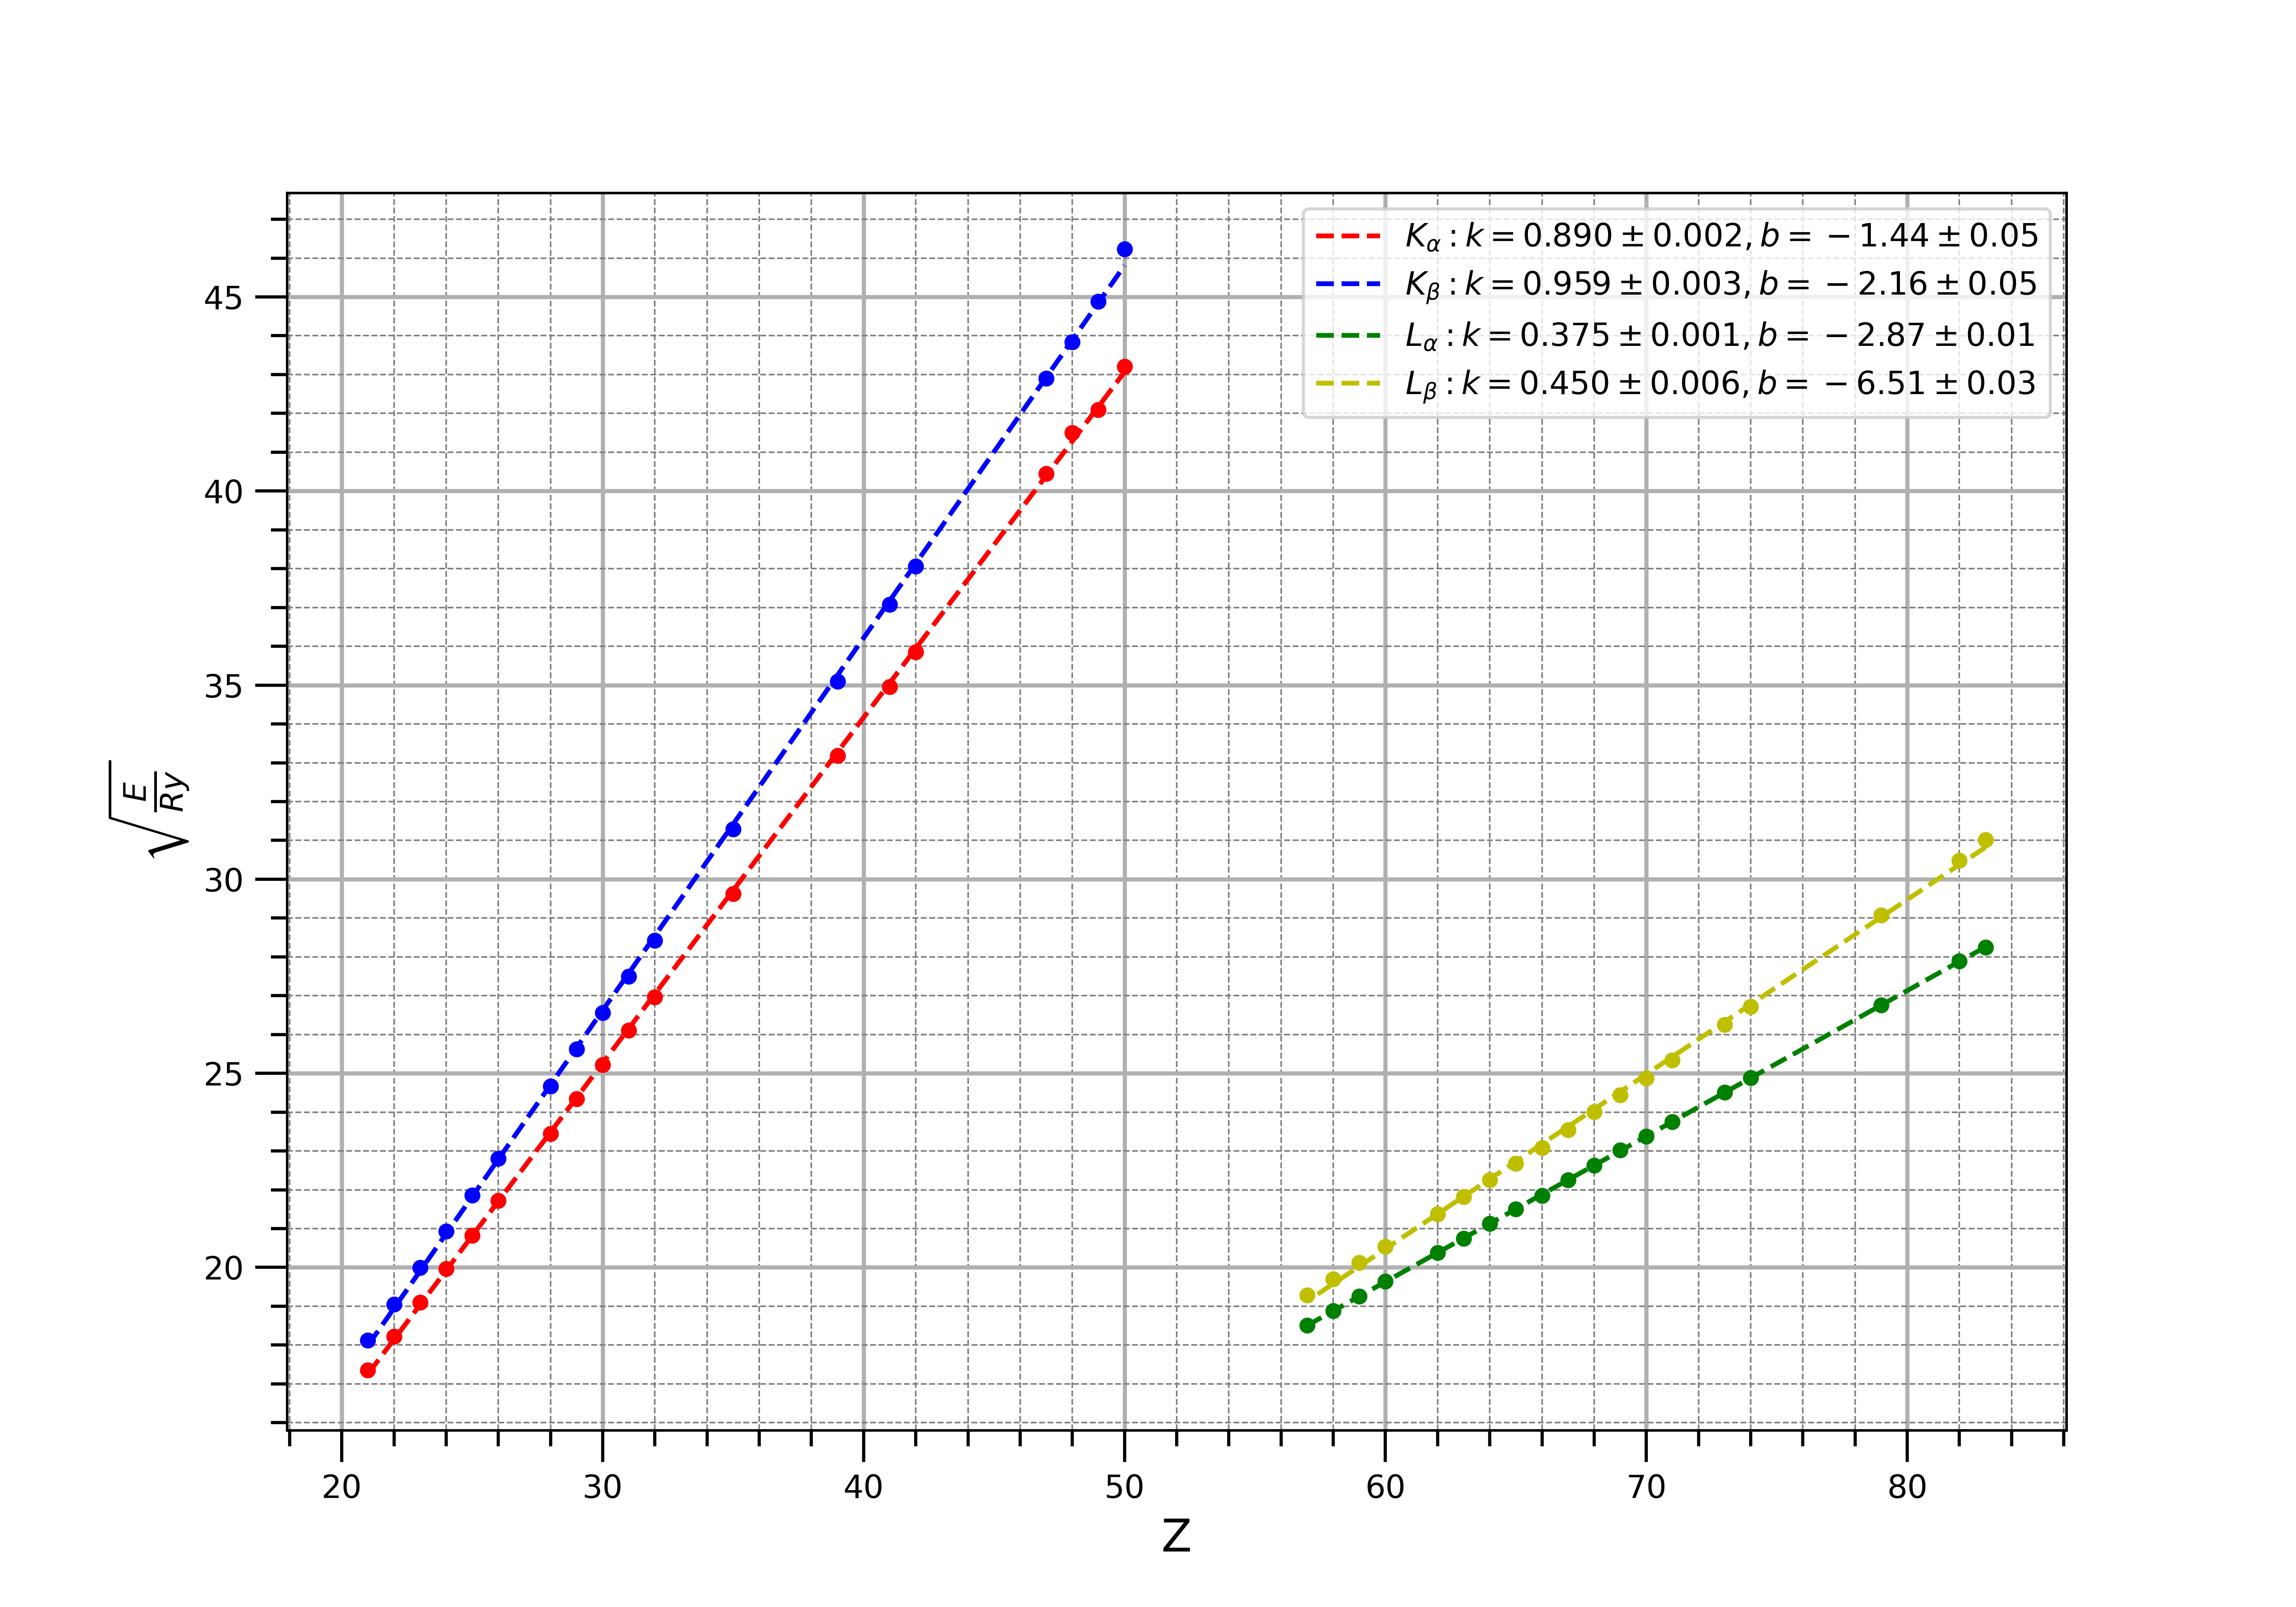
\includegraphics[scale=0.8]{ERy(z).png}}
			\caption{График зависимости величины $\sqrt{\frac{E}{Ry}}$ от атомного номера Z. Произведена аппроксимация методом наименьших квадратов. По построенным прямым определены коэффициенты их наклона k и точки пересечения b с осью ординат}
		\end{figure}
		
		
		
		
		
		
		
		
		
		
		
		
		
		
		
		
		
		
		
		
		
		
		
		
		
		
	\end{enumerate}
	
	
	
	
	
	
	
	
	
	
	
	
	
	
	\end{document}
